\subsection{wiringPi}
Der NanoPi Neo2 Black kommt mit einem vorinstallierten Fork von der wiringPi Libarry
https://github.com/friendlyarm/WiringNP/blob/master/wiringPi/wiringPi.c
Die funktionalität der drei verwendetetn C-Funktionen werden im folgenden beschrieben.
\subsubsection{wiringPiI2CSetup}

Der Funktion wird beim audfruf die I2C Adresse übergeben mit welcher eine verbindung aufgebaut werden soll: wiringPiI2CSetup(address).\\
Der Rückgabewert ist der Standard Linux File Disciptor oder -1, falls ein Fehler auftritt. 
Die Anzahl der File Desciptoren ist begrenzt daher muss die verbindung mit der Funktion close() aus der Library: unistd.h geschlossen werden wenn sie nicht mehr benötigt wird.


\subsubsection{wiringPiI2CWriteReg8}
Der Funktion wird bei aufruf der File Desciptor einer I2C verbindung sowie ein ziel register und die zu schreibenden 8bit Daten übergeben: wiringPiI2CWriteReg8 (fd, RegAdr, 8-Bit-Data).
Wenn der Schreibzugriff vom I2C gerät bestätigt wurde wird eine 0 zurück gegeben.
\subsubsection{wiringPiI2CReadReg8}
Der Funktion wird bei aufruf der File Desciptor einer I2C verbindung sowie ein ziel register übergeben: wiringPiI2CReadReg8(fd, RegAdr).
Der ausgelsene 8-Bit inhalt des Register ist der rüchgabewert.
Wenn das Lesen Fehlschlägt bleibt das Programm in einer Endlosschleife hängen.

\subsection{AS726X Libary}
Die WiringPi\_AS726X\_Libary enthält alle funktionen um den AS7261 und AS7265X zu steuern und auszulesen.
Da die Beispielimplementierungen im Datenblatt in vielen detaifragen ungenau und Fehlerhaft ist wurde die Arduino OpenSource Libarrys von sparkfun SparkFun\_AS726X\_Arduino\_Library-master und SparkFun\_AS7265x\_Arduino\_Library als implementierungs grundlage verwendet.
Im ersten schritt der entwirklung wurde sie für die I2C schnittschelle WiringPi des NanoPi umgeschrieben und anschließen in ihrer Funktionalität erweitert um für das messystem mit mehreren sensoren auf dem gleichen bus nutzbar zu sein. \\

Im Folgenden Text werden die Register Adressen und mit den gleichen Namen wie im source code bezeichnet die Numerische Adressen sind in Tabelle \ref{TODO} aufgelistet. TODO table

\begin{figure}[H]
\centering
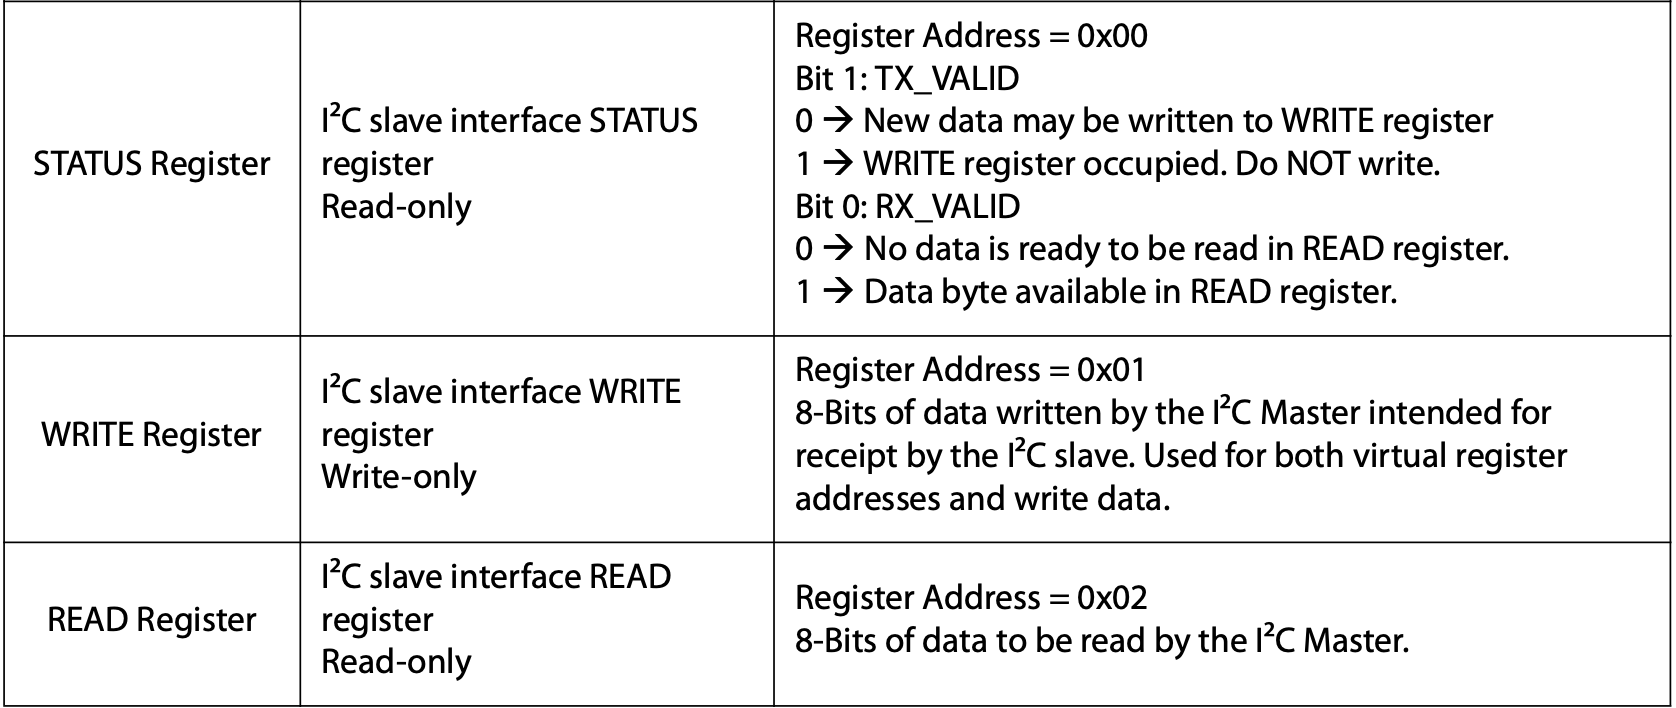
\includegraphics[width=0.75\textwidth]{img/PysicalRegister}
%\caption*{Quelle: Datenblatt AS7261}
\caption{PysicalRegister}
\label{fig:Seitenasicht-AS726X}
\end{figure}

\begin{figure}[H]
\centering
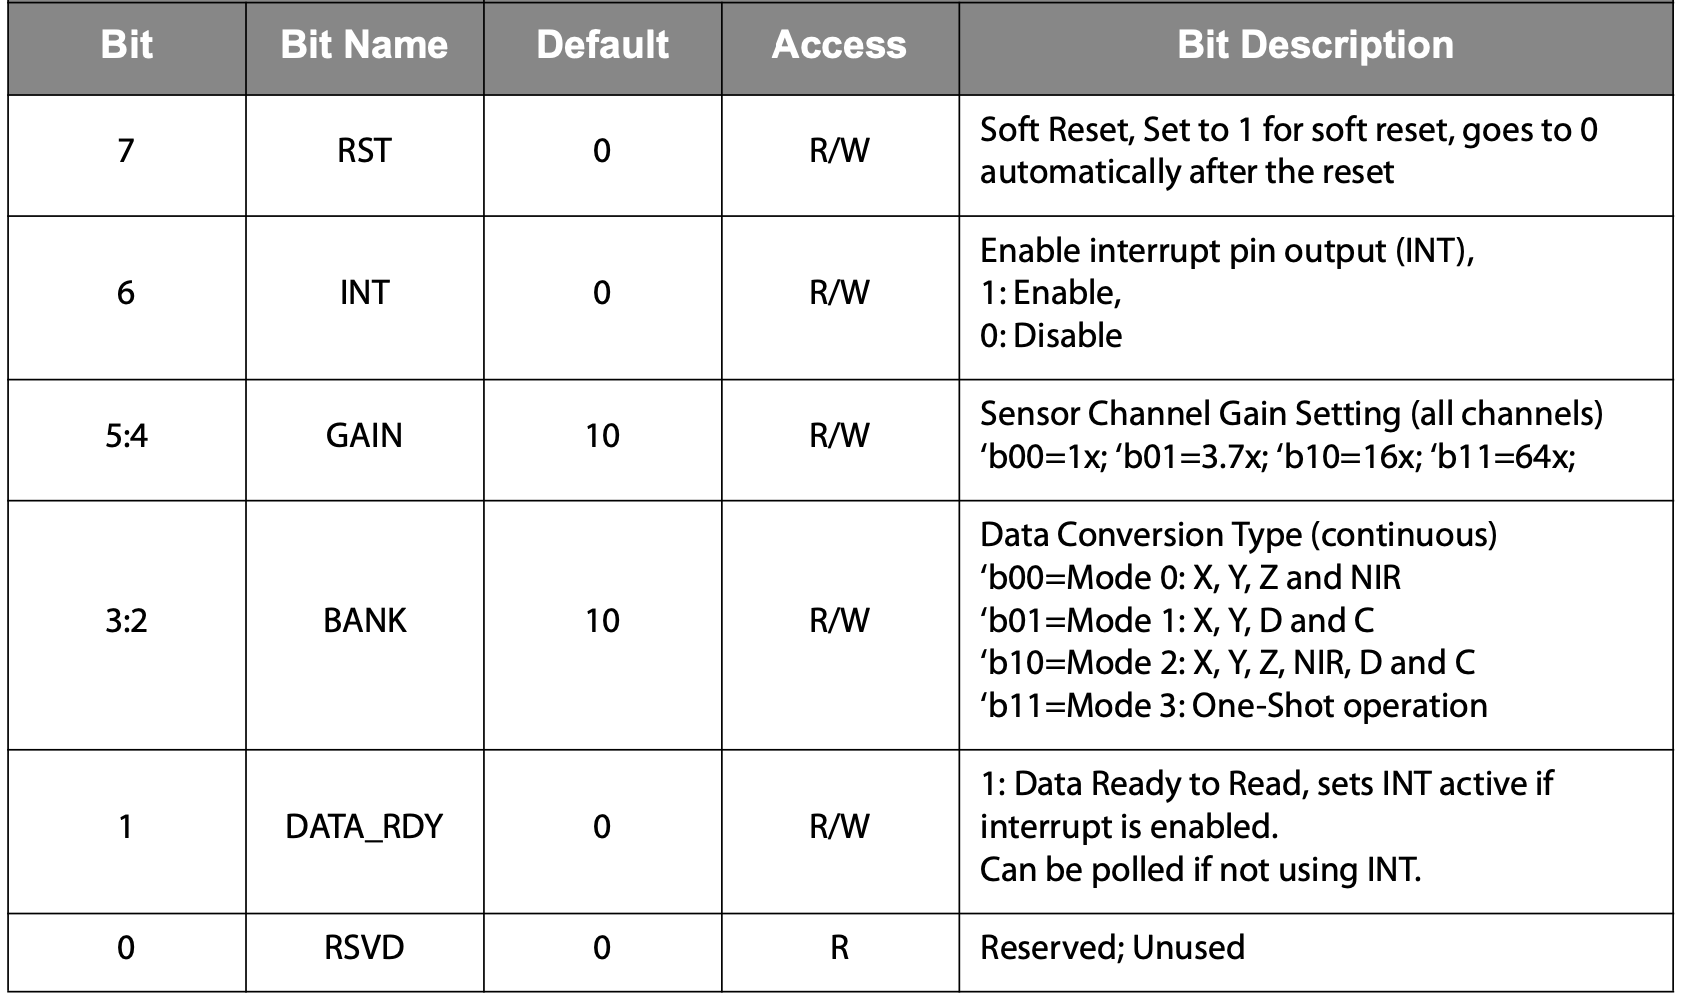
\includegraphics[width=0.75\textwidth]{img/ControlRegister_2}
%\caption*{Quelle: Datenblatt AS7261}
\caption{AS726x\_CONTROL\_SETUP}
\label{fig:Seitenasicht-AS726X}
\end{figure}

\subsubsection{virtualWriteRegister}
Wie bei Embeddet geräten üblich werden Einstellungen auf dem sensor verändern indem verschiedene sogenannte Special function registers  mit daten beschrieben werden.\\
Jedes Special function register ist 8Bit groß und hat eine adresse und
jedes Bit des Register representiert eine einstellung.
Beispielsweise ist 0x07 das LED Control Register des Sensors.
Bit 0 des Registers Beschreibt den Zustand der Status LED.
Die Restlichen 7 Bit des Registers Beschreibt den Zustand anderer LEDs die für den Messaufbau aber irrelevant sind.\\
Wird register 7 mit dem Dezimal wert 0 beschrieben sind alle LED aus, wird es mit dem Dezimal wert 1 beschrieben leuchtet ist nur die status LED.
Die Register Lassen sich aber nicht direkt Beschreiben, stattdesswen sind sie als sogennate Virtuelle Register Implementiert.

Der Sensor arbeitet mit virtuellenRegistern.
Das heißt das nur Register 0x01 (WRITE Register) beschrieben werden kann.
Um daten in eins der Special Funktions Register zu schreiben wird die funktion virtualWriteRegister verwendet.
Die Funtionsweise lässt sich in 4 schritten zusammnefassen:
\begin{itemize}
	\item Zeile TODO Warten bis das WRITE Register leer ist, was angezeigt wird indem  das Bit AS72XX\_TX\_VALID im  Register AS72XX\_STATUS\_REG den wert 1 annimmt.
	\item Zeile TODO Schreibe die Virtuelle Adresse in das WRITE Register und Setze zusätzlich Bit 8 des WRITE Register auf 1 um zu zeigen das es sich um einen Schreibenden zugriff auf das Virtuelle Register handelt.
	\item Warte erneut bis das WRITE Register leer ist.
	\item Schreibe die Daten in das WRITE Register
\end{itemize}
Der Sensor wird jetzt selber die übertragenen Daten aus dem WRITE Register angebene Virtuelle Register kopieren.
\lstinputlisting[language=C,style=c]{code/virtualWriteRegister.c}
\subsubsection{virtualReadRegister}
Die Unterschiedlichen Messdaten des Sensors werden in dedizierten registern gespeichert.
 Es ist aber nur über den indirekten weg des AS72XX\_READ\_REG und der Virtuellen Register Adressen möglich daten auszulesen.
Die Funktionsweise der zum Daten auslesen benötigten funktion virtualReadRegister lässt sich wieder in 4 schritte aufteilen.
\begin{itemize}
	\item Das AS72XX\_READ\_REG wird ausgelesen ohne das die daten verabeitet werden. Dieser schritt ist wie ein Reset des Registers zu verstehen.
	\item Zeile TODO Schreibe die Virtuelle Adresse in das WRITE Register und Setze zusätzlich Bit 8 des WRITE Register auf 0 um zu zeigen das es sich um einen Lesenden zugriff auf das Virtuelle Register handelt.
	\item Sobald das AS72XX\_STATUS\_REG den wert AS72XX\_TX\_VALID annimmt sind die Daten aus dem angebenen Virtuellen Register in das AS72XX\_READ\_REG kopiert worden.
	\item Lese die Daten aus dem S72XX\_READ\_REG
\end{itemize}
\lstinputlisting[language=C,style=c]{code/virtualReadRegister.c}

\subsubsection{MeasurementFromAdress}
Die Funktion baut einen I2C Verbindung zur übergebenen Bus-Adresse auf und  ruft die Funktion takeMeasurments mit dem File Descriptor der aktiven I2C Verbindung auf.
Nachdem die Funktion takeMeasurements durchlaufen ist wird die I2C Verbindung wieder geschlossen.
\lstinputlisting[language=C,style=c]{code/MeasurementFromAdress.c}

\subsubsection{takeMeasurements}

Die Funktion takeMeasurements ruft die Funktion setMeasurementMode mit dem Parameter 3 auf das setzt den aus \ref{todo} bekannten Bankmode der übergebenen I2C Verbindung (fd) auf Bank Mode 3.
	Die On-Shot Messung wird sofort gestartet, in Zeile 9 wird gewartet bis die Messung abgeschlossen ist. 
		Um sicherzustellen das die funktion DataAvailable richtig arbeitet muss vor der Messung das Flag DataAvailable auf 0 gesetzt werden (Zeile 3).
Die Daten werden hier nicht ausgelesen daher gibt es keinen rückgabewert.\\
\lstinputlisting[language=C,style=c]{code/takeMeasurements.c}

\subsubsection{setMeasurementMode}
Mit der Funktion setMeasurementMode werden die Bankmode Bits 2 und 3 des AS726x\_CONTROL\_SETUP Registers mit dem gewünschten wert für den Bankmode beschrieben.\\
Da die anderen Bits des Registers noch weitere einstellungen repräsentieren welche nicht verändert werden sollen, muss das register erst ausgelsen werden.
Anschließend werden die Bankmode Bits auf 0 gesetzt um im nächsten schritt mit dem gewünschten neuen Bankmode wert beschrieben zu werden. 
Die Bedeutung der Bankmodes ist in \ref{TODO} erleutert.
\lstinputlisting[language=C,style=c]{code/setMeasurementMode.c}
\subsubsection{dataAvailable \& clearDataAvailable}
Das Bit dataAvailble im register todo wird vom Sensor auf 1 gesetzt wenn nach einer Messung neue daten vorhanden sind, Intterupts müssen dafür ausgeschaltet sein.
dataAvailble wird auf 0 gesetzt wenn daten gelsen werden.
Wenn eine One-Shot messung im Bankmode 3 durchgeführt wird sollte das dataAvailble bit mit der Funktion clearDataAvailable auf 0 gesetzt werden, da nicht sicher gestellt ist das die daten vor der Messung gelsen wurden. Es besteht die möglichkeit das sich das bit fälschicherweise noch im falsch positiven zustand befindet.
Die Funktion dataAvailable gibt den wert des DataAvailable Bit zurück.
\lstinputlisting[language=C,style=c]{code/dataAvailable.c}
\subsection{Rohwerte des AS7261 Auslesen}
Die in \ref{todo} beschrieben 6 Channel des AS7261 werden mit den folgenden Funktionen ausgelesen:
\begin{itemize}
	\item getX\_CIE(fd)
	\item getY\_CIE(fd)
	\item getZ\_CIE(fd)
	\item getNIR(fd)
	\item getDark(fd) 
	\item getClear(fd)
\end{itemize}
Der File Diskritor einer I2C verbindung mit einem AS7261 wird als übergabe parameter erwatet.\\
Um den Messert auszulesen wir die Funktion getchannel aufgerufen.
Der Rückgabewer ist der 16-Bit Messwert aus dem jewaligen Register vom Datentyp Integer.

\subsection{getChannel}
Da die Messdaten 16-Bit groß sind, der Sensor aber nur über 8 Bit register verfügt werden 2 aufeinader folgende register ausgelsen und im Big-Andian Format aneinader geheftet.
Die Funktion getChannel erwatet einen File Disciptor einer I2C verbindung zu einem Sensor und die adressen des High Bytes Raw Data Registers.

\subsection{disableInterrupt}
Die Funktion disableInterrupt setzt das INT Bit im register AS726x\_CONTROL\_SETUP auf 0 um Interrupts aus zu schalten.
Da Der Interrupt auf der Sensor Paltiene nicht verbinden ist muss .. toto muss dass wirklich?


